
\section{BETTER PRACTICES FOR BODY BIASING INJECTION}
%\begin{frame}
%    \frametitle{Why working with BBI?}
%    \begin{itemize}
%        \setlength\itemsep{1em}
%        \item BBI introduced to perform Bellcore attack;
%        \item Demanding fault attacks difficult or impossible to perform;
%        \item Low experiment repeatability.
%    \end{itemize}
%    \vspace{1cm}
%    \begin{center}
%        \huge What are the limiting factors?
%    \end{center}
%\end{frame}

\begin{frame}
    \frametitle{State-of-the-art BBI platform: limiting factors}
    \begin{columns}
        \begin{column}{0.33\textwidth}
            \centering
            \begin{figure}
                
\includegraphics[width=1.0\textwidth]{model0Probe.pdf}
            \end{figure}
            \vspace{-0.5cm}
            \begin{figure}
                \includegraphics[width=0.9\textwidth]{S1P.pdf}\\
                \includegraphics[width=0.9\textwidth]{S1G.pdf}
            \end{figure}
        \end{column}
        \barsep
        \begin{column}{0.67\textwidth}
%            \centering
%            \begin{itemize}
%                \setlength\itemsep{1em}
%                \item Impedance mismatch → Ringing and set-point error
%                \item Floating grounds → Set-point error
%            \end{itemize}
            \begin{textblock*}{120mm}(65mm, 20mm)
                • Impedance mismatch → Ringing and set-point error\\
                • Floating grounds → Set-point error
            \end{textblock*}
            \begin{textblock*}{55mm}(60mm, 30mm)
                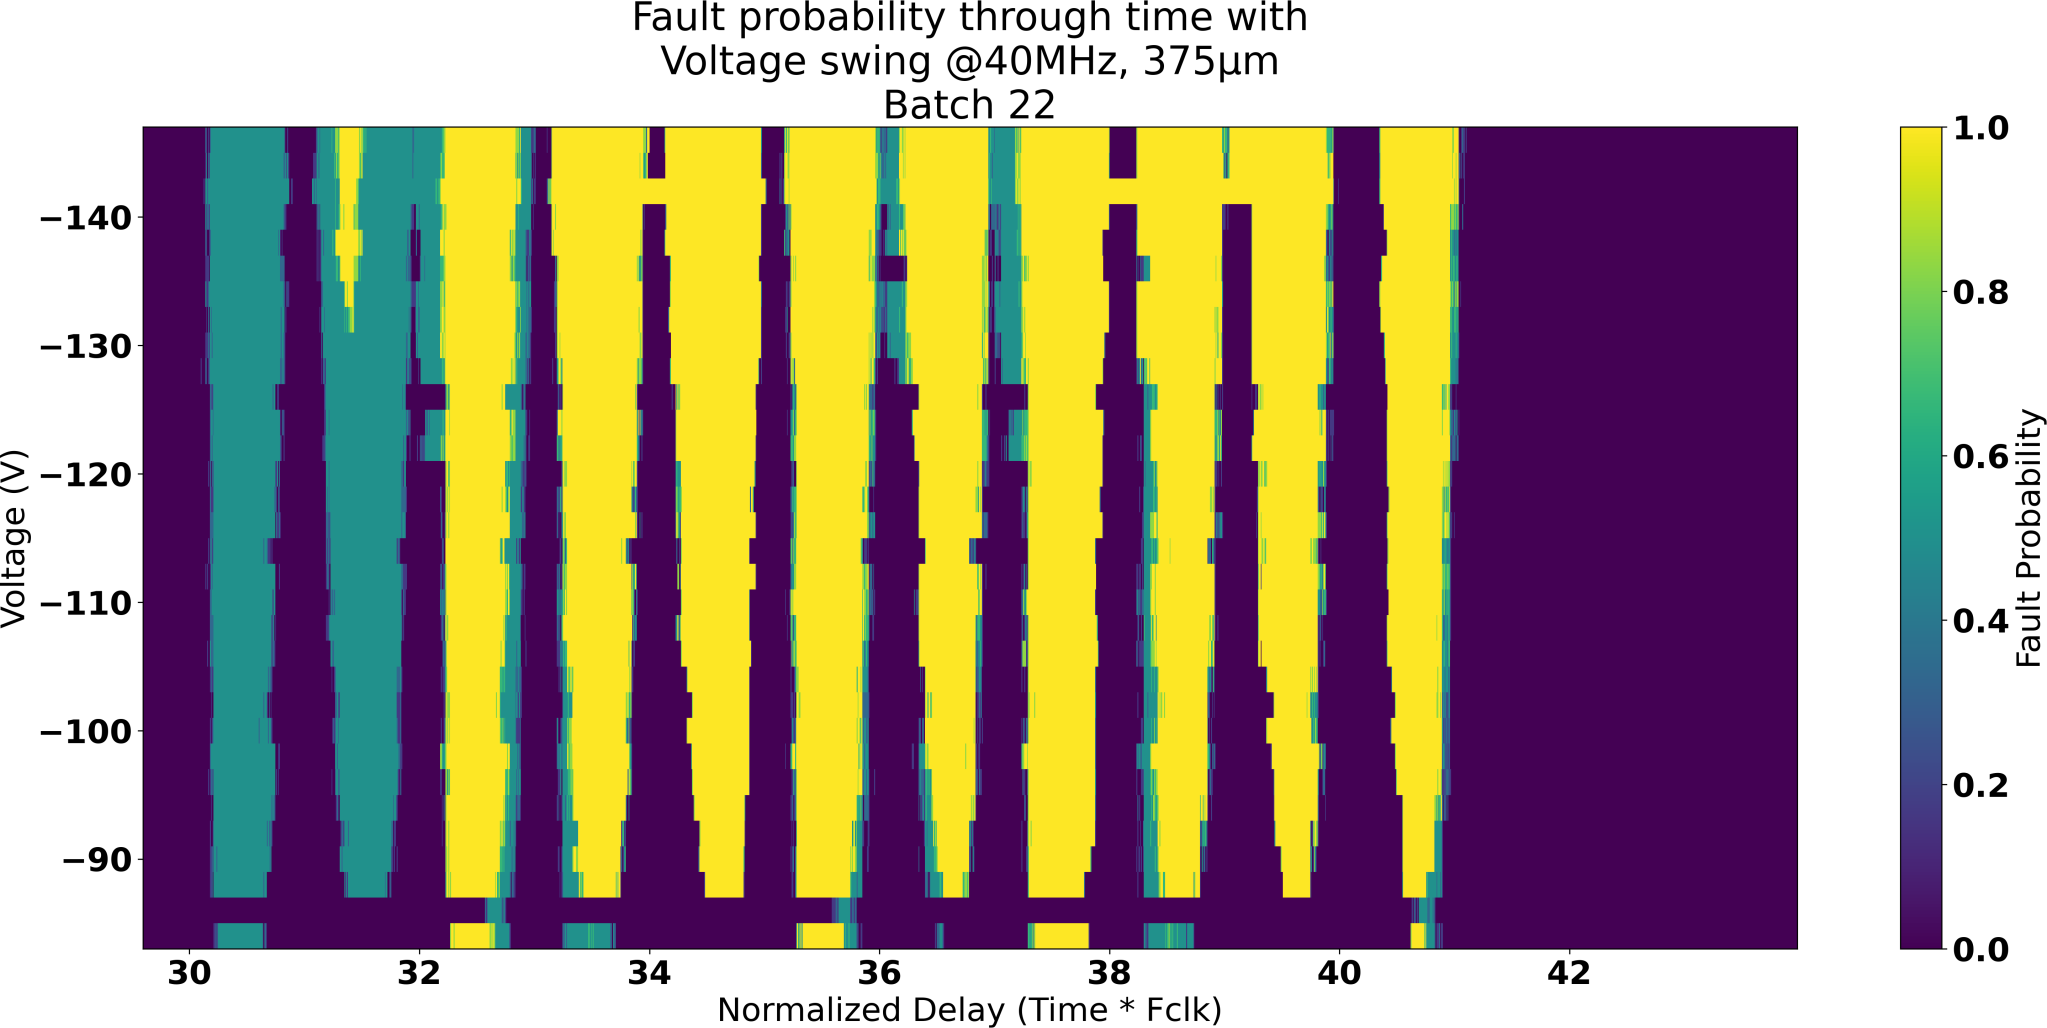
\includegraphics[width=\textwidth]{probafautes0.png}
            \end{textblock*}
            \begin{textblock*}{55mm}(100mm, 55mm)
                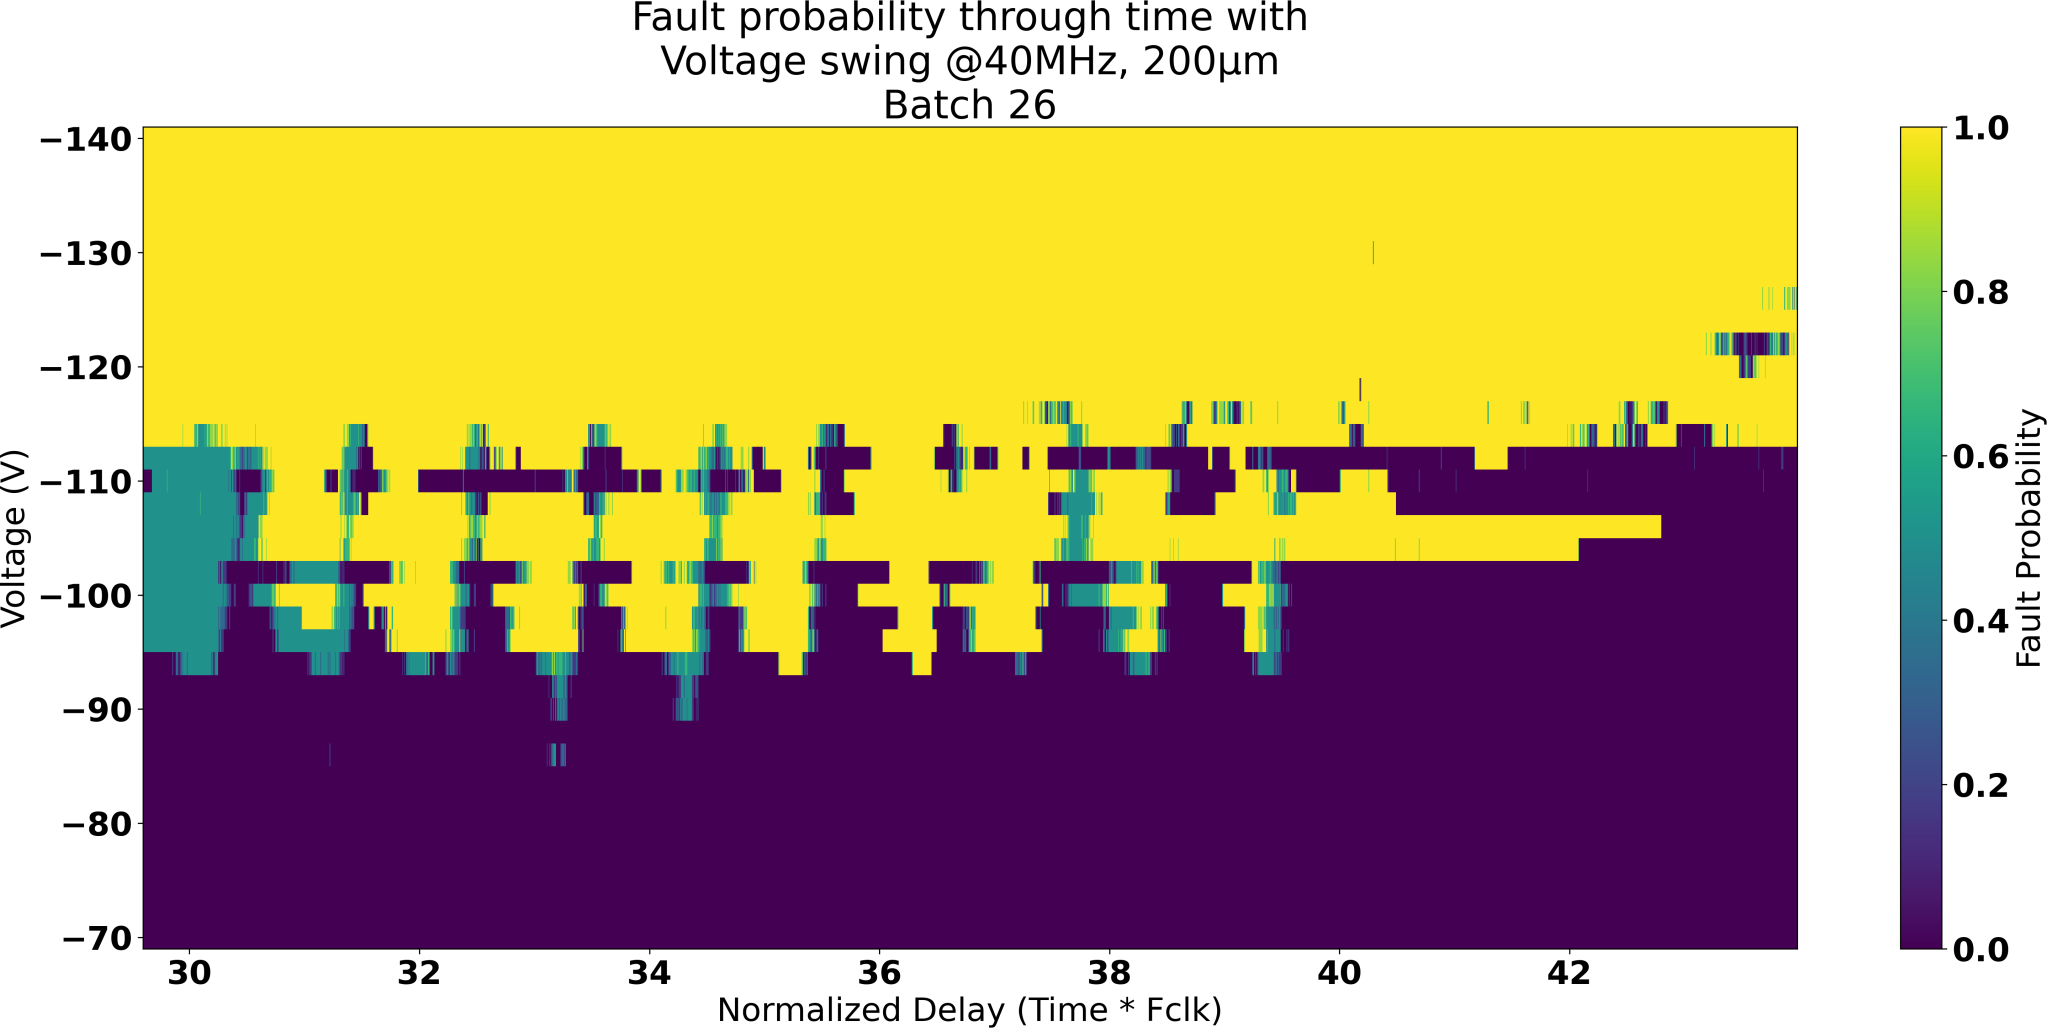
\includegraphics[width=\textwidth]{probafautes1.png}
            \end{textblock*}
        \end{column}
    \end{columns}
\end{frame}
